%%%%%%%%%%%%%%%%%%%%%%%%%%%%%%%%%%%%%%%%%%%%%%%%%%%%%%%%%%%%%%%%%%%%%%%%%%%%%%%%%%
\begin{frame}[fragile]\frametitle{}
\begin{center}
{\Large From Zero to GPT!!}
\end{center}
\end{frame}

%%%%%%%%%%%%%%%%%%%%%%%%%%%%%%%%%%%%%%%%%%%%%%%%%%%%%%%%%%%%%%%%%%%%%%%%%%%%%%%%%%
\begin{frame}[fragile]\frametitle{}
\begin{center}
{\Large ``Houston, we have a problem!!''}
\end{center}
\end{frame}

%%%%%%%%%%%%%%%%%%%%%%%%%%%%%%%%%%%%%%%%%%%%%%%%%%%%%%%%%%%%%%%%%%%%%%%%%%%%%%%%%%
\begin{frame}[fragile]\frametitle{Whats the Problem?}
\begin{itemize}
\item Along with some softer words like ``disruption'', ``passionate'', ``excited'' \ldots
\item If you don't have word ``innovation'' in your talk/speech/conversation it's  BIG problem. 
\item Irrespective of fields. You can be Corporate, Political, Social, etc.
\end{itemize}


And there is an addition of one more word,  which is a must in every talk...and that is?


\end{frame}

%%%%%%%%%%%%%%%%%%%%%%%%%%%%%%%%%%%%%%%%%%%%%%%%%%%%%%%%%%%%%%%%%%%%%%%%%%%%%%%%%%
\begin{frame}[fragile]\frametitle{}
\begin{center}
{\Large ``AI''}
\end{center}
\end{frame}


%%%%%%%%%%%%%%%%%%%%%%%%%%%%%%%%%%%%%%%%%%%%%%%%%%%%%%%%%%%
\begin{frame}[fragile]\frametitle{The Problem}
Every company is claiming to be working in AI-ML
\begin{itemize}
\item Is it really so?
\item What exactly is AI (ML)?
\item What is not AI?
\end{itemize}
Or is it just a plain BIG hype?
\end{frame}


%%%%%%%%%%%%%%%%%%%%%%%%%%%%%%%%%%%%%%%%%%%%%%%%%%%%%%%%%%%%%%%%%%%%%%%%%%%%%%%%%%
\begin{frame}[fragile]\frametitle{}
\begin{center}
{\Large What is the Core Idea?}
\end{center}
\end{frame}


%%%%%%%%%%%%%%%%%%%%%%%%%%%%%%%%%%%%%%%%%%%%%%%%%%%%%%%%%%%%%%%%%%%%%%%%%%%%%%%%%%
\begin{frame}[fragile]\frametitle{What's the core idea?'}
\begin{itemize}
\item behind problem solving?
\item behind writing software algorithms?
\item solving research problems?
\end{itemize}
\end{frame}

%%%%%%%%%%%%%%%%%%%%%%%%%%%%%%%%%%%%%%%%%%%%%%%%%%%%%%%%%%%
\begin{frame}[fragile]\frametitle{Desire}
\begin{itemize}
\item To find a ``function''
\item To find a relation
\item To find a transformation
\item To build a model
\item From given inputs to desired outputs.
\end{itemize}
That's it.
\end{frame}


%%%%%%%%%%%%%%%%%%%%%%%%%%%%%%%%%%%%%%%%%%%%%%%%%%%%%%%%%%%
\begin{frame}[fragile]\frametitle{Functions}
\begin{itemize}
\item But most real-life functions are not deterministic
\item Some are probabilistic, some non-linear.
\item {\em ``Detecting if the tumor is benign or malignant''}
\item {\em ``At any state in the game of chess, whats the next move?''}
\end{itemize}
\end{frame}

%%%%%%%%%%%%%%%%%%%%%%%%%%%%%%%%%%%%%%%%%%%%%%%%%%%%%%%%%%%
\begin{frame}[fragile]\frametitle{Chess: next move?}
\begin{itemize}
\item Needs extreme expertise
\item Needs ``intelligence''
\item How do you get that?
\begin{itemize}
\item Built by lots of training.
\item By studying lots of past games.
\end{itemize}
\item This is how Humans build intelligence
\end{itemize}
\end{frame}

%%%%%%%%%%%%%%%%%%%%%%%%%%%%%%%%%%%%%%%%%%%%%%%%%%%%%%%%%%%
\begin{frame}[fragile]\frametitle{Intelligence}
\begin{itemize}
\item Can machine (software/program) also do the same?
\item Can it play chess?
\item Can it build intelligence?
\item By looking at past experiences (data), 
\item Training Data: games played, moves used, etc.
\end{itemize}
Yes, it can!! Thats Artificial Intelligence.
\end{frame}


%%%%%%%%%%%%%%%%%%%%%%%%%%%%%%%%%%%%%%%%%%%%%%%%%%%%%%%%%%%
\begin{frame}[fragile]\frametitle{Relationship between AI, ML, DL}
\begin{center}
\includegraphics[width=\linewidth,keepaspectratio]{ai1}
\end{center}
{\tiny (Ref: https://blogs.nvidia.com/blog/2016/07/29/whats-difference-artificial-intelligence-machine-learning-deep-learning-ai/)}
\end{frame}

%%%%%%%%%%%%%%%%%%%%%%%%%%%%%%%%%%%%%%%%%%%%%%%%%%%
\begin{frame}[fragile] \frametitle{What is AI-ML-DL?}

\begin{itemize}
\item Artificial Intelligence: mimicking human intelligence
\item Machine Learning: Automating Learning with features. 
\item ML: human-designed representations and input features.  So, its just optimizing weights to best make a final prediction
\item There could be programmed (hand coded) AI, that's not Machine Learning
\item Machine Learning could be for non AI activities, like automation
\item Deep Learning: Neural network with no input features
\end{itemize}
\end{frame}


%%%%%%%%%%%%%%%%%%%%%%%%%%%%%%%%%%%%%%%%%%%%%%%%%%%%%%%%%%%%%%%%%%%%%%%%%%%%%%%%%%
\begin{frame}[fragile]\frametitle{}
\begin{center}
{\Large Introduction to Machine Learning}
\end{center}
\end{frame}

%%%%%%%%%%%%%%%%%%%%%%%%%%%%%%%%%%%%%%%%%%%%%%%%%%%%%%%%%%%
\begin{frame}[fragile]\frametitle{How do we learn?}
\begin{itemize}
	\item What do we do when we have to prepare for an examination? 
	\item Study. Learn. Imbibe. Take notes. Practice mock papers.
	\item  Thus,  prepare for the unseen test.
	\item Machine Learning does the same.
\end{itemize}
\end{frame}



%%%%%%%%%%%%%%%%%%%%%%%%%%%%%%%%%%%%%%%%%%%%%%%%%%%%%%%%%%
\begin{frame}[fragile]\frametitle{What is Machine Learning?}
Machine learning is a type of artificial intelligence (AI) which:
\begin{itemize}
\item Learns function without being explicitly programmed. 
\item Can grow and change when exposed to new data. 
\end{itemize}
\end{frame}


%%%%%%%%%%%%%%%%%%%%%%%%%%%%%%%%%%%%%%%%%%%%%%%%%%%%%%%%%%%
\begin{frame}[fragile]\frametitle{Model entities}
For $income = c + \beta_0 \times education + \beta_1 \times experience$
\begin{itemize}
\item Inputs: Education and experience, also called as features or attributes or dimensions or variables.
\item Mathematical entities added to input data, are Parameters.. $\beta_0$ and $\beta_1$ are parameters
\item Income is target, also called as outcome or class.
\end{itemize}
\end{frame}

%%%%%%%%%%%%%%%%%%%%%%%%%%%%%%%%%%%%%%%%%%%%%%%%%%%%%%%%%%%
\begin{frame}[fragile]\frametitle{Traditional vs. Machine Learning?}
\begin{center}
\includegraphics[width=0.8\linewidth,keepaspectratio]{tradml}
\end{center}
\end{frame}


%%%%%%%%%%%%%%%%%%%%%%%%%%%%%%%%%%%%%%%%%%%%%%%%%%%%%%%%%%%
\begin{frame}[fragile]\frametitle{Why Machine Learning?}
\begin{itemize}
\item Problems with High Dimensionality
\item Hard/Expensive to program manually
\item Techniques to model `ANY' function given `ENOUGH' data.
\item Job \$\$\$
\end{itemize}
%\begin{center}
%\includegraphics[width=0.45\linewidth,keepaspectratio]{hp}
%\end{center}
\end{frame}



%%%%%%%%%%%%%%%%%%%%%%%%%%%%%%%%%%%%%%%%%%%%%%%%%%%
\begin{frame}[fragile] \frametitle{ML vs DL: What's the difference?}
Deep learning algorithms attempt to learn (multiple levels of) representation by using a hierarchy of multiple layers
\begin{center}
\includegraphics[width=\linewidth,keepaspectratio]{dlfeat1}
\end{center}
\tiny{(Reference: https://www.xenonstack.com/blog/static/public/uploads/media/machine-learning-vs-deep-learning.png)}

\end{frame}

%%%%%%%%%%%%%%%%%%%%%%%%%%%%%%%%%%%%%%%%%%%%%%%%%%%%%%%%%%
\begin{frame}[fragile] \frametitle{Use Deep Learning When \ldots}

\begin{itemize}
\item You have lots of data (about 10k+ examples)
\item The problem is ``complex'' - speech, vision, natural language
\item The data is unstructured 
\item You need the absolute ``best'' model
\end{itemize}
\tiny{(Ref: Introduction to TensorFlow 2.0 - Brad Miro)}
\end{frame}


%%%%%%%%%%%%%%%%%%%%%%%%%%%%%%%%%%%%%%%%%%%%%%%%%%%%%%%%%%%
\begin{frame}[fragile]\frametitle{What is Deep NLP}
\begin{center}
\includegraphics[width=0.8\linewidth,keepaspectratio]{nlp4}

\tiny{(Ref: Deep Learning and NLP A-Z - Kirill Eremenko)}

\tiny{(Note: Size is not indicative of importance)}
\end{center}

	\begin{itemize}
	\item Green part is NLP (rule based, linguistic)
	\item Blue part is Deep Learning not applied to NLP
	\item Purple is Deep NLP (DNLP), NN applied for NLP use cases
	\item Seq2Seq is heavily used technique of DNLP for sequence to sequence modeling, eg Translation, Q \& A, etc.
	\end{itemize}
	

\end{frame}


%%%%%%%%%%%%%%%%%%%%%%%%%%%%%%%%%%%%%%%%%%%%%%%%%%%%%%%%%%%
\begin{frame}[fragile]\frametitle{Typical Machine Learning Classification}
	\begin{itemize}
	\item Questions are converted to bag of words (a vocab long vector, having frequency of specific words at their places)
		\item Each question thus gets converted to fixed size vector, which acts as list of features.
		\item In training, weights are computed based on the given target.
		\item Once model is ready, it is able to answer Yes or No to the question.
			\end{itemize}
\begin{center}
\includegraphics[width=0.6\linewidth,keepaspectratio]{nlp11}

\tiny{(Ref: Deep Learning and NLP A-Z - Kirill Eremenko)}
\end{center}

\end{frame}


%%%%%%%%%%%%%%%%%%%%%%%%%%%%%%%%%%%%%%%%%%%%%%%%%%%%%%%%%%%
\begin{frame}[fragile]\frametitle{Context}

Representing words by their context

\begin{center}
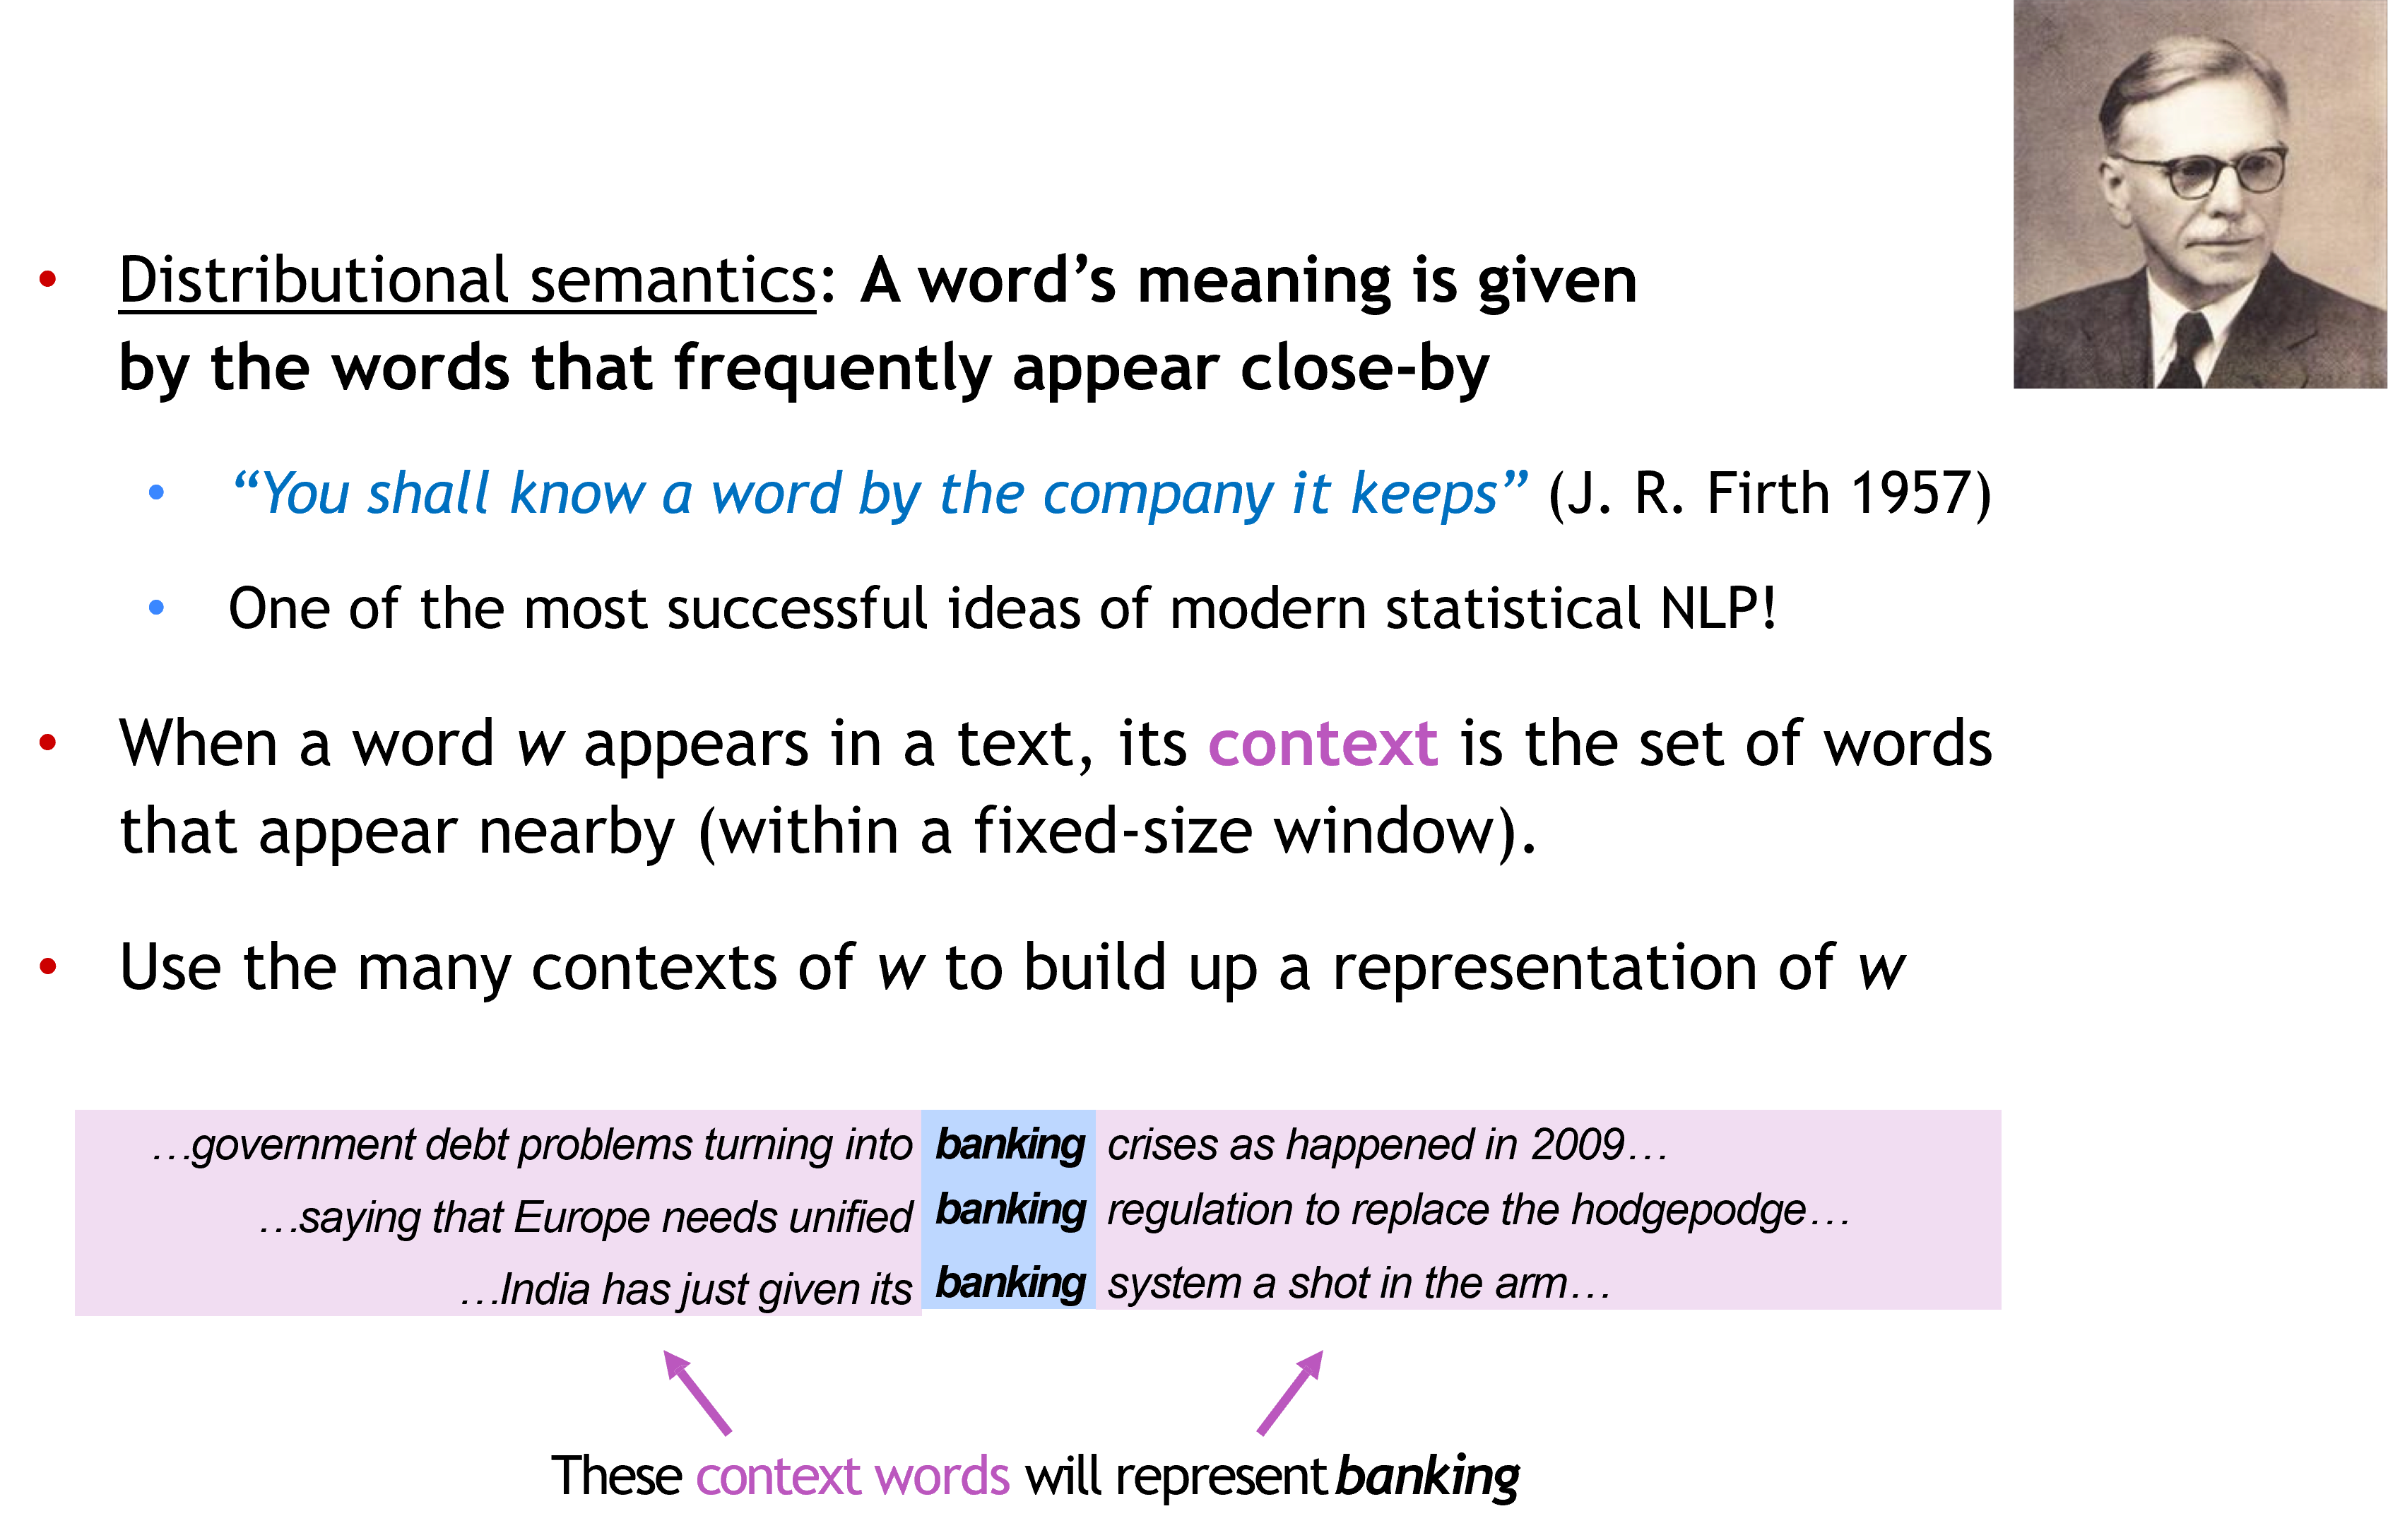
\includegraphics[width=\linewidth,keepaspectratio]{bert6}
\end{center}		  


{\tiny (Ref: CS224n: Natural Language Processing with Deep Learning - Christopher Manning)}

\end{frame}

%%%%%%%%%%%%%%%%%%%%%%%%%%%%%%%%%%%%%%%%%%%%%%%%%%%%%%%%%%%
\begin{frame}[fragile]\frametitle{Word vectors}

\begin{columns}
    \begin{column}[T]{0.5\linewidth}
			\begin{itemize}
			\item Dense vector for each word
			\item Called distributed representation, word embeddings or  word representations 
			\item Test: similar to vectors of words that appear in similar contexts
			\end{itemize}
    \end{column}
    \begin{column}[T]{0.5\linewidth}
			\begin{center}
			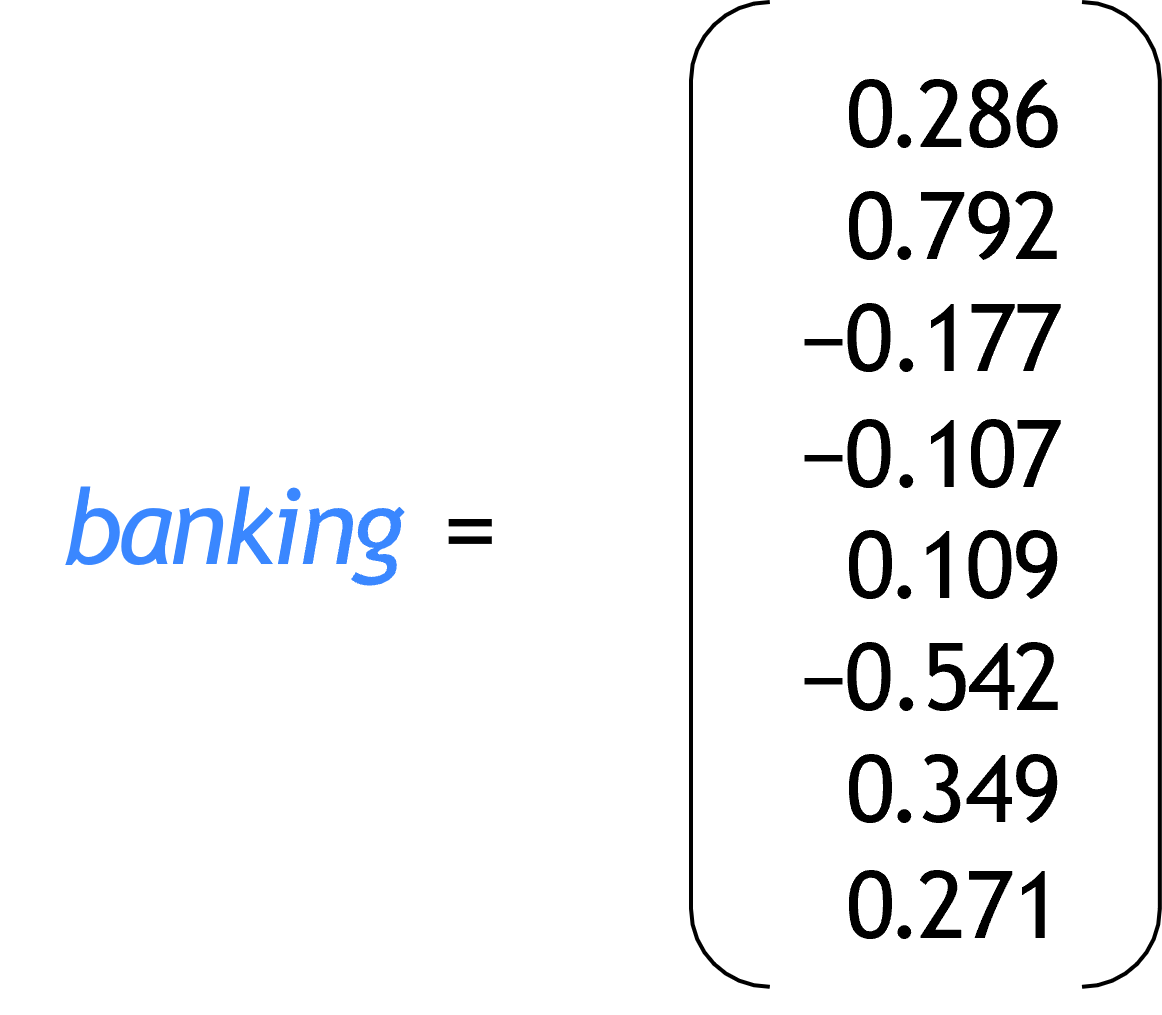
\includegraphics[width=0.4\linewidth,keepaspectratio]{bert7}
			\end{center}		  
    \end{column}
  \end{columns}
% {\tiny (Ref: CS224n: Natural Language Processing with Deep Learning - Christopher Manning)}

\end{frame}
% %%%%%%%%%%%%%%%%%%%%%%%%%%%%%%%%%%%%%%%%%%%%%%%%%%%%%%%%%%%
% \begin{frame}[fragile]\frametitle{Seq2Seq architecture}

% \begin{center}
% \includegraphics[width=\linewidth,keepaspectratio]{nlp13}

% \tiny{(Ref: Deep Learning and NLP A-Z - Kirill Eremenko)}
% \end{center}

% For Seq2seq last 2 options are possible. We are going ahead with the 2nd last. Last one has fixed input and same size output.

% \end{frame}

%%%%%%%%%%%%%%%%%%%%%%%%%%%%%%%%%%%%%%%%%%%%%%%%%%%%%%%%%%%
\begin{frame}[fragile]\frametitle{Seq2Seq architecture}

\begin{center}
\includegraphics[width=0.8\linewidth,keepaspectratio]{nlp14}

\tiny{(Ref: Deep Learning and NLP A-Z - Kirill Eremenko)}
\end{center}
During training, Encoder is fed with Questions and decoder with Answers. Weights in gates, hidden states get settled. During testing for each sequence of input, encoder results in to a combo vector. Decoder takes this and starts spitting out words one by  one, probabilistically.

\end{frame}


% %%%%%%%%%%%%%%%%%%%%%%%%%%%%%%%%%%%%%%%%%%%%%%%%%%%%%%%%%%%
% \begin{frame}[fragile]\frametitle{Popularity}

% Masking the future in self-attention

% \begin{center}
% 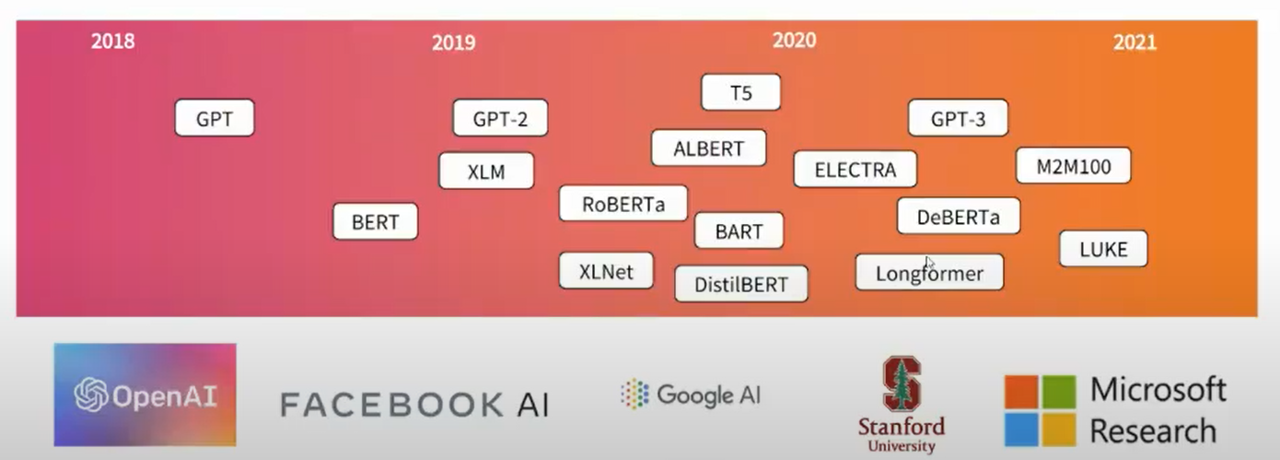
\includegraphics[width=\linewidth,keepaspectratio]{bert50}
% \end{center}	

 
% % {\tiny (Ref: Niels Rogge on Huggingface contributions)}
% \end{frame}


%%%%%%%%%%%%%%%%%%%%%%%%%%%%%%%%%%%%%%%%%%%%%%%%%%%%%%%%%%%
\begin{frame}[fragile]\frametitle{Transformers}


\begin{itemize}
\item The Transformer  is a model that uses attention to boost the speed with which seq2seq with attention models can be trained. The biggest benefit, however, comes from how The Transformer lends itself to parallelization. 
\item In its heart it contains an encoding component, a decoding component, and connections between them.
\end{itemize}	 

\begin{center}
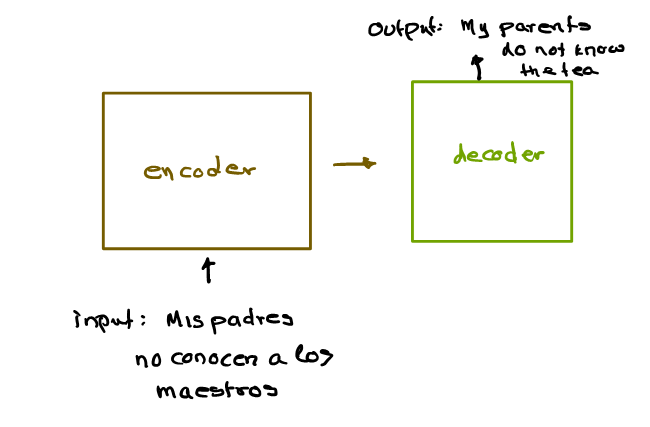
\includegraphics[width=0.6\linewidth,keepaspectratio]{bert51}
\end{center}	

\end{frame}

%%%%%%%%%%%%%%%%%%%%%%%%%%%%%%%%%%%%%%%%%%%%%%%%%%%%%%%%%%%
\begin{frame}[fragile]\frametitle{Transformers}


\begin{itemize}
\item Offer a better structure to train a language model, which gave raise to the large language models (LLMs) like GPT and Bart. Its characteristics are:
\begin{itemize}
\item Positional encoding: each word is labeled with the number of its position in a sentence.
\item Self-attention: each word is examined in the context of the whole sentence to generate a representation of the word. This helps the model to understand the linguistic meaning and nuances of a word.
As the scale of a language model grows, the model builds mastery of our human language, and it does not only know how to perform basic text-based tasks but also gives a structured and logical answer to any user prompt.
\end{itemize}	 
\end{itemize}	 

{\tiny (Ref: Techy Stuff 1: Notes on Transformers, LLMs, and OpenAI - Bill)}
\end{frame}

%%%%%%%%%%%%%%%%%%%%%%%%%%%%%%%%%%%%%%%%%%%%%%%%%%%%%%%%%%%%%%%%%%%%%%%%%%%%%%%%%%
\begin{frame}[fragile]\frametitle{}
\begin{center}
{\Large GPT}
\end{center}
\end{frame}


%%%%%%%%%%%%%%%%%%%%%%%%%%%%%%%%%%%%%%%%%%%%%%%%%%%%%%%%%%%
\begin{frame}[fragile]\frametitle{Generative Pretrained Transformer (GPT)}



2018’s GPT was a big success in pretraining a decoder!


      \begin{itemize}
			\item Transformer decoder with 12 layers.
			\item 768-dimensional hidden states, 3072-dimensional feed-forward hidden layers.
			% \item Byte-pair encoding with 40,000 merges
			\item Trained on BooksCorpus: over 7000 unique books.
			\item Contains long spans of contiguous text, for learning long-distance dependencies.
			\item The acronym ``GPT'' never showed up in the original paper; it could stand for
			\item ``Generative PreTraining'' or ``Generative Pretrained Transformer''
			\end{itemize}

			
			{\tiny (Ref: John Hewitt, Radford et al., 2018)}

\end{frame}

%%%%%%%%%%%%%%%%%%%%%%%%%%%%%%%%%%%%%%%%%%%%%%%%%%%%%%%%%%%
\begin{frame}[fragile]\frametitle{GPT-3, in-context learning, very large models}


      \begin{itemize}
			% \item So far, we’ve interacted with pretrained models in two ways:
			      % \begin{itemize}
						% \item Sample from the distributions they define (maybe providing a prompt)
						% \item Fine-tune them on a task we care about, and take their predictions.
						% \end{itemize}
			\item Very large language models seem to perform some kind of learning without gradient  steps simply from examples you provide within their contexts.
			\item GPT-3 is the canonical example of this. The largest T5 model had 11 billion parameters.
			\item GPT-3 has 175 billion parameters.

			\end{itemize}

			{\tiny (Ref: John Hewitt)}

\end{frame}





